\chapter{Conexión a interfaz del sistema hotelero}\label{chapter:Conexion a interfaz del sistema hotelero}

		En este capítulo se describe el proceso general que fue llevado a cabo para el desarrollo del módulo de conexión a la interfaz IFC8, software mediante el cual se pueden extraer los datos necesarios de los huéspedes del hotel. La primera sección se refiere a la instalación y configuración del servidor de interfaces. En la segunda sección se detalla el proceso del levamiento de un socket para establecer la comunicación con dicho servidor. En la tercera sección se exponen los mensajes en el protocolo FIAS, que deben ser enviados para completar el proceso. Y finalmente, en la cuarta sección, se resumen los resultados obtenidos en esta fase del proyecto.

\section{Instalación y configuración del servidor de interfaces} \label{sect:Instalacion y configuracion del servidor de interfaces}
	El primer paso para establecer la comunicación con IFC8 fue instalar la aplicación  correspondiente en un servidor Windows Server 2008 R2 Enterprise, de 64 bits y 1GB de memoria RAM. La configuración correcta estuvo a cargo de un consultor de la empresa propietaria Oracle Micros-Opera, en la que se estableció FIAS como protocolo de comunicación. De igual forma, se definieron los puertos de conexión, por los cuales la comunicación con el PMS se haría efectiva. Es relevante mencionar que este proceso se pudo ejecutar luego de obtener la licencia pertinente, por parte de Oracle Micros-Opera.

\section{Levantamiento de \textit{socket}}
	Una vez instalada la aplicación en el servidor designado, se procedió a entablar los primeros intercambios de información entre NetPass y dicho servidor de interfaces, por lo que fue necesaria la creación de una clase denominada NetPassSocket, que como su nombre lo indica se encargó de la gestión de envío y recibo de ‘mensajes’ entre NetPass e IFC8, a través de un socket de tipo SOCKSTREAM. Esto debido a que el protocolo de comunicación entre ambos entes, es TCP. 

\section{Mensajes FIAS enviados}
		FIAS (acrónimo de Fidelio Interface Application Specification, por sus siglas en inglés), es el protocolo estándar de comunicación de interfaces IFC8, y especifica claramente los mensajes que dicha interfaz es capaz de reconocer. Existen cuatro tipos de mensajes que establecen la conexión, en el siguiente orden: Link Record, Link Start, Link Description y Link Alive. Un cambio en el orden de envío de dichos mensajes produce que no se establezca la comunicación adecuadamente. Por otra parte, están presentes los mensajes que pueden ser enviados solo si la comunicación se efectuó correctamente. Estos son: Database Resync Request y Post Simple, cuya función es pedir al PMS una sincronización de su base de datos, y enviar una solicitud de cobro al PMS, respectivamente.
\newline
\newline		
\indent Al inicio y final de cada mensaje existen caracteres necesarios para que el mensaje esté completo, e IFC8 lo entienda. Dichos caracteres no tienen una representación clara en la pantalla de la interfaz IFC8, por lo que fue pertinente la utilización de un software analizador del tráfico de la red denominado Wireshark, para determinar su traducción. El analizador determinó que el  caracter de inicio se traduce a \textbackslash x02 y, el caracter final a \textbackslash x03. 
\\
\newline
\indent En la Tabla ~\ref{table:ejFias} se muestran los mensajes FIAS, enviados a IFC8. Mientras en que la tabla  ~\ref{table:ejFiasRec} se muestran los mensajes FIAS recibidos de IFC8.

\begin{table}[H]
%\centering 
\begin{tabular}{ p{6cm} p{10cm} }
\hline 
\bfseries \footnotesize {Nombre} & \bfseries \footnotesize {Mensaje} \\ 
\hline
\footnotesize {Link Alive} &\footnotesize  LA$\vert$DA160601$\vert$TI151500$\vert$
\\ \hline
\footnotesize {Link Start} &\footnotesize  LS$\vert$DA160601$\vert$TI151500$\vert$ \\ \hline
\footnotesize {Link Description} &\footnotesize LD$\vert$DA160601$\vert$TI151500$\vert$VFIAS:3.1$\vert$IFWW$\vert$RT130$\vert$\\ \hline
\footnotesize {Link Record GuestIn} &\footnotesize LR$\vert$RIGI$\vert$FLDATIRNG\#GNGVGLGS$\vert$
 \\ \hline
\footnotesize {Link Record GuestOut} &\footnotesize LR$\vert$RIGO$\vert$FLDATIRNG\#GNGVGSSF$\vert$\\  \hline  
\footnotesize {Data Resync} &\footnotesize DR$\vert$DA160601$\vert$TI151500$\vert$\\  \hline 
\footnotesize {Link End} &\footnotesize LE$\vert$DA160601$\vert$TI151500$\vert$\\  \hline 
\footnotesize {Post Simple} &\footnotesize PS$\vert$DA160601$\vert$TI151500$\vert$RN$\vert$TA$\vert$PT$\vert$\\  \hline 
\end{tabular}
\footnotesize \caption{Tabla de mensajes FIAS enviados a IFC8}
\label{table:ejFias}
\end{table}


\begin{table}[H]
%\centering 
\begin{tabular}{ p{3cm} p{13cm} }
\hline 
\bfseries \footnotesize {Nombre} & \bfseries \footnotesize {Mensaje} \\ 
\hline
\footnotesize {Link Start} &\footnotesize  LS$\vert$DA160601$\vert$TI151500$\vert$ \\ \hline
\footnotesize {Guest-In} &\footnotesize  GI$\vert$DA160601$\vert$TI151500$\vert$RN651$\vert$G\#13862439$\vert$GNAntoun$\vert$GVVIP5$\vert$GLSP$\vert$GSN$\vert$
\\ \hline
\footnotesize {Guest-Out} &\footnotesize  GO$\vert$DA160601$\vert$TI151500$\vert$RN651$\vert$G\#13862439
$\vert$GNAntoun$\vert$GVVIP5$\vert$GSN$\vert$SFN$\vert$
\\ \hline
\end{tabular}
\footnotesize \caption{Tabla de mensajes FIAS recibidos de IFC8}
\label{table:ejFiasRec}
\end{table}

\section{Resultados obtenidos}
		Como resultado de esta etapa del desarrollo se obtuvo el módulo de conexión a la interfaz del sistema hotelero. En este punto, el sistema es capaz de especificar a la interfaz, las ‘consultas’ a la base de datos del sistema hotelero que quiere ejecutar. En respuesta, el PMS, mediante la interfaz, provee lo solicitado.
		
	En la Figura ~\ref{fig:estsyn} se muestra un ejemplo del mensaje que envía IFC8, al recibir la notificación del ingreso de un huésped (check-in), y su respectiva leyenda.

\begin{figure}[ht]
  \centering
  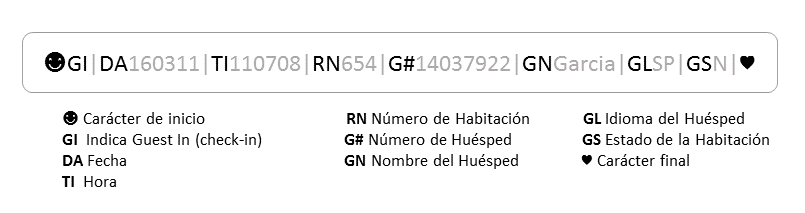
\includegraphics[scale=0.6,type=png,ext=.png,read=.png]{imagenes/ejemploDetallado} \\
  \caption{Ejemplo de mensaje recibido al registrar el check-in de un huésped.}
  \label{fig:estsyn}
\end{figure}

\section{Pruebas}
			Una vez finalizado el desarrollo de este módulo, la metodología MSF nos conduce a realizar las pruebas unitarias correspondientes. Estas consistieron en la transmisión de mensajes mediante el shell interactivo de Python, evaluando el formato en el que la interfaz los envíaba.